%% Copernicus Publications Manuscript Preparation Template for LaTeX Submissions
%% ---------------------------------
%% This template should be used for copernicus.cls
%% The class file and some style files are bundled in the Copernicus Latex Package, which can be downloaded from the different journal webpages.
%% For further assistance please contact Copernicus Publications at: production@copernicus.org
%% https://publications.copernicus.org/for_authors/manuscript_preparation.html


%% Please use the following documentclass and journal abbreviations for preprints and final revised papers.

%% 2-column papers and preprints
\documentclass[tc, manuscript]{copernicus}

\usepackage{placeins}



\begin{document}

\title{Response to Reviewer 1 for "Snow accumulation variability limits InSAR SWE retrieval"}


% \Author[affil]{given_name}{surname}

\Author[1][zmhoppinen@alaska.edu]{Zachary}{Hoppinen} %% correspondence author
\Author[1]{Simon}{Zwieback}
\Author[2]{Ross}{Palomaki}
\Author[3]{Hans-Peter}{Marshall}

\affil[1]{Geophysical Institute, University of Alaska Fairbanks, 2156 Koyukuk Drive, Fairbanks, AK}

% \affil[1]{Institute of Arctic and Alpine Research, University of Colorado, 4001 Discovery Dr, Boulder, CO 80303, USA}
\affil[2]{Institute of Arctic and Alpine Research, University of Colorado, 4001 Discovery Dr, Boulder, CO 80303, USA}
\affil[3]{Department of Geosciences, Boise State University, 1910 University Drive, Boise, ID 83725, USA}

\runningauthor{Z. Hoppinen et al.}
\runningtitle{Response to Reviewer 1}

\maketitle


\textit{
This is a very interesting and timely analysis of the limitations of InSAR SWE retrieval. The authors provide great motivation for this study and tie it to snow applications relatable to Cryosphere readers. It is unique in its focus on specific InSAR processing effects over complex terrain where the underlying snow depth and water content distributions are highly variable. The validation study with aerial lidar is appropriate and well thought out. My main overall comment is that this is very heavy in remote sensing theory and the general Cryosphere audience could use more context and explanation, especially as this relates to NISAR. The Theoretical Framework section assumes a lot of familiarity with SAR and InSAR processing at a level that some, used to polished science data products, may lack. I think much of this could be resolved with the inclusion of one or more figures that help explain the windows, multi-look windows, averaged windows, and sub-windows, and how these relate to the "pixels" we'd see in a NISAR data product. The Discussion section does a great job capturing the major points and takeaways for other researchers.}

Thank you for taking the time to read and give this thoughtful review of our paper. Find each point addressed below. Line numbers refer to the revised draft.

\textbf{Specific Comments}

\textit{Theory (2): I would like a graphical representation that clearly explains the windows, multi-look windows, averaged windows, and sub-windows. The concept of windows is brought up with little context, and at first I was confusing it between spatial and temporal windowing. For the science user base interacting with NISAR data, it would be nice also graphically explain the relation between these window definitions and pixels. If multi-look averaging is a step in NISAR's data processing I'd like to see a more detailed description of it. I'm not sure if it is using adjacent frames from along NISAR's orbit or a pair of SAR collections. Is Figure 1 showing sub-windows that end up as a single pixel in an InSAR data product?}

Thank you, we appreciate this is a central idea and worth the space to explain clearly. We have added an example figure (Figure 1) showing the spatial averaging and window sizes using a zoom from the December pair of NISAR acquisitions. Section 2 now opens with a paragraph that defines the resolution cell, the multi-look window, and the product pixel, and states the two window sizes NISAR uses for its 20\,m and 80\,m layers (lines 75--81). Yes, each panel of the phasor figure (now Figure~2) is one multi-look window that becomes one pixel of the product, and its caption now says so.

\begin{figure}
    \centering
    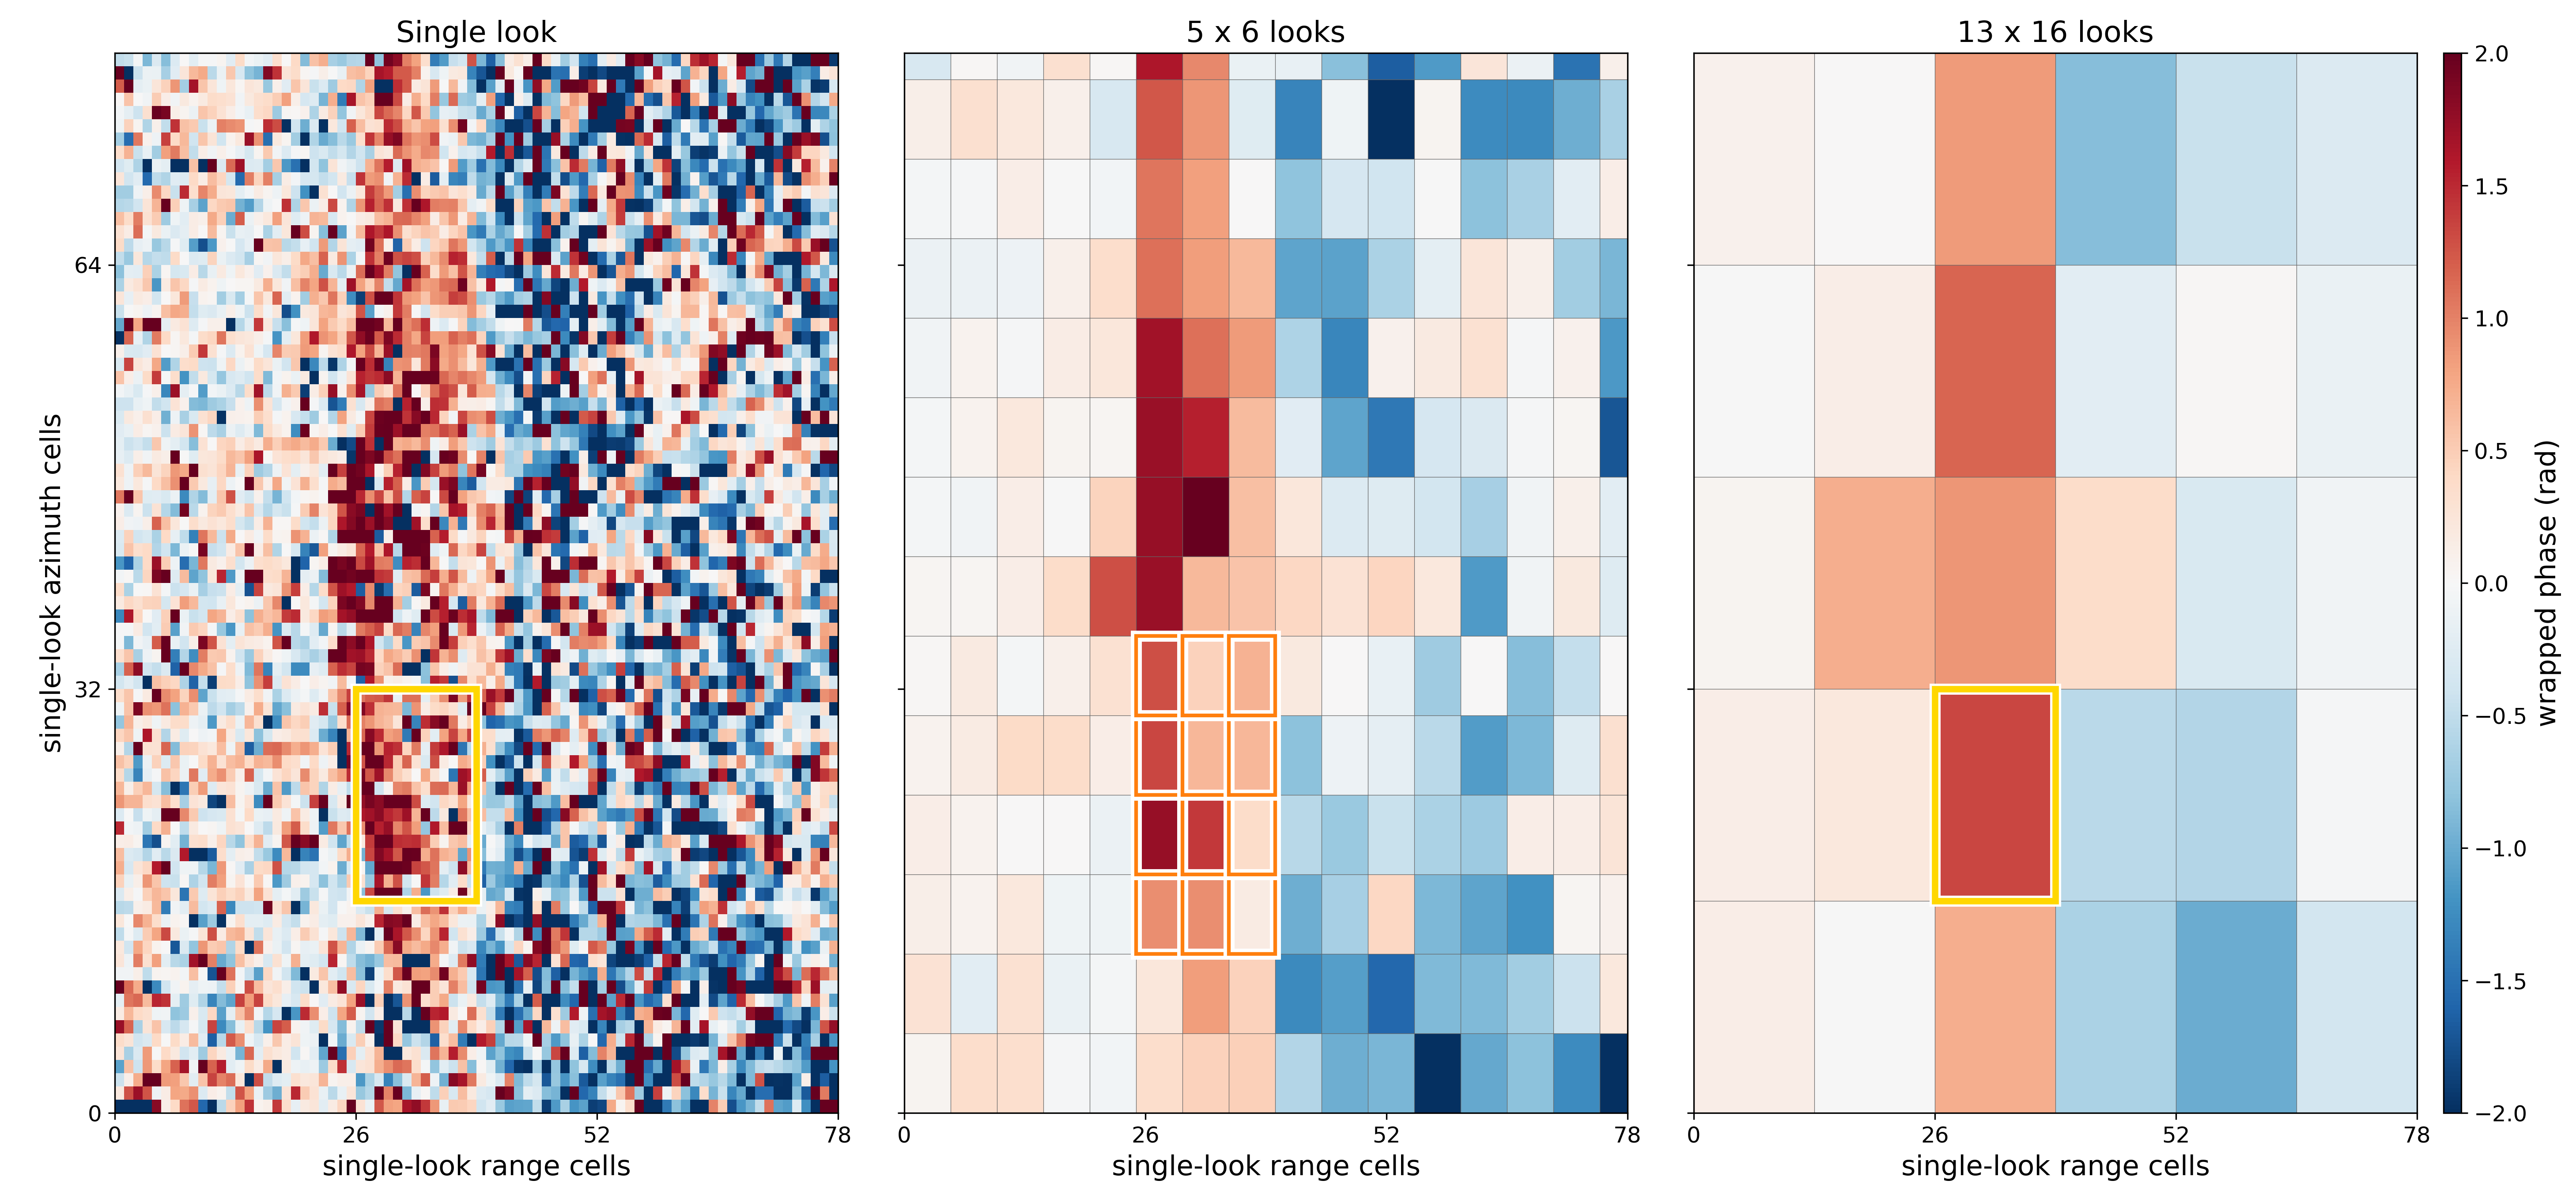
\includegraphics[width=0.5\linewidth]{figures/0_multilook_windows.png}
    \caption{Manuscript Figure 1}
    \label{fig:placeholder}
\end{figure}

\textit{Theory (2): I would consider not setting φ=Δφ since it is used so few times, and Section 3.4 seems to revert to the Δφ notation.}

We agree and have removed the $\phi = \Delta\phi$ shorthand. Section 2, including Equations 2 and 3 and the Figure~2 caption, now uses $\Delta\phi$ throughout, matching the Introduction and Section 3.4 (lines 90--99).

\textit{Methods (3.1, 3.2): Can we get more information on the LiDAR system used, i.e. the platform and sensor, flight height, GNSS positioning? Also, define how snow depth and SWE are calculated. I assume snow depth comes from digital terrain differencing, but what algorithms are used? And why do snow depth and SWE have different resolutions (3m and 50m)?}

Yes, here are some details from the two papers we could find and an email response from ASO. We have added citations describing the ASO lidar system and products to Section 3.2 (lines 158--161) and expand with more detail here, based on Painter et al. (2016) and updated details provided by ASO (J. Deems, personal communication, 2026). The flights used here (2023--2026) were collected with a Riegl VQ-1560 II-S airborne laser scanner, positioned with a lidar-integrated Trimble Applanix AP60 GNSS/IMU differentially corrected with Applanix RTX. Each survey is flown at a constant altitude, generally 5800--7300\,m (19,000--24,000\,ft) above sea level, so the height above ground and the ground point density varies with the terrain.

Snow depth is computed by subtracting gridded snow-free surfaces from gridded snow-on surfaces. Following Section 5.2.2 of Painter et al. (2016), separate surface pairs are built from first returns in open terrain and from ground points classified under forest canopy, and the two resulting depth grids are merged using vegetation masks. SWE is the product of snow depth and a bulk snow density simulated by the iSnobal model, which assimilates the observed snow depth map and adjusts based on in-situ density observations.

ASO grids snow depth at 3\,m from the lidar data, while SWE is delivered at 50\,m, the resolution of the iSnobal model that simulates the snow density. We use the finer 3\,m depth to keep the most spatial detail and convert it to $\Delta$SWE with a density taken from the 50\,m products (Section 3.2).

We don't include the emailed information in the main text as The Cryosphere discourages personal communication citations.

\textit{Methods (3.3): Provide a graphical representation of the radial power spectral density for ΔSWE spatial variation.}

This figure already exists as Figure~5 (Figure~3 of the original submission), which shows the radial power spectral density of the $\Delta$SWE field for every 1.15\,km window with the fitted two-segment power law and the break wavelength. It was placed with the results, but Section 3.3 did not point to it. Section 3.3 now refers to it where the radial spectrum is introduced (line 170).

\textit{Methods (3.3): How is 95\% snow cover determined? Is this what Appendix B covers? If so, specify.}

The 95\% criterion comes from the lidar snow mask, not from the VIIRS snow cover of Appendix B. A window is kept for the spectral analysis when at least 95\% of its cells pass the lidar snow test of Section 3.2 in all four pairs. Section 3.3 now states this (line 179). Appendix B uses VIIRS only as an independent check on the snow coverage from the NISAR coherence residual.

\textit{Methods (3.4): How is κ calculated?}

We use the dry-snow approximation of Leinss et al. (2015), $\kappa = (2\pi/\lambda)(1.59 + \theta^{5/2})$ with $\theta$ in radians, which gives 52.7, 224.1 and 15.5\,rad\,m$^{-1}$ of $\Delta$SWE at L-, C- and P-band for the 40$^\circ$ incidence angle used throughout. Section 3.4 now states the formula as Eq.~(9) and the wavelength and incidence angle it is evaluated at (lines 200--202). Leinss et al. (2015) include a correction factor $\alpha$ that they set to 1. We omit it rather than introduce a symbol only to remove it.

\textit{Methods (3.5): arg(M) and κ have been described, but the introduction of arg(M)/κ could use more description.}

$\arg(M)$ is a phase, and dividing by $\kappa$ turns it into an SWE error. Section~2.1 now defines $|M|$ as the coherence factor and $\arg(M)$ as the retrieval bias, the offset of the averaged phase from the phase of the window-mean $\Delta$SWE (lines 126--128), and Section~3.5 refers back to it where $\arg(M)/\kappa$ is reported.

\textit{Methods (3.6): Again, a figure showing how multi-looking works specifically for NISAR would be helpful for potential NISAR users.}

The new Figure~1 shows this for NISAR directly. Section 3.6 now refers to it where the 5$\times$6 and 13$\times$16 look counts are introduced (line 250). The single-look interferogram in that figure was formed from the delivered NISAR RSLCs with the same ISCE3 workflow that produces the standard GUNW (see the related repository for the code), but with the multi-looking step turned off, so the three panels differ only in the window size.

\textit{Methods (3.6): In Equation 9, what does the $\tilde{{}}$ over γ mean for true coherence? One line 199 true coherence was called simply γ.}

The tilde marks the bias-corrected estimate of the true coherence $\gamma$, obtained by inverting the Bamler and Hartl (1998) expectation, and the hat the sample coherence delivered in the product. Section~3.6 now defines all three where Eq.~(12) is introduced (lines 264--266), and the corrected difference is written $\tilde{\gamma}_{20}-\tilde{\gamma}_{80}$ throughout.

\textit{Results: Figure 4, indicate where there is higher elevation / more complex terrain, perhaps in a separate figure of the basin.}

We have added a study area figure (new Figure~3) in Section 3.1 showing elevation with hillshade over the lidar coverage, along with the CDEC snow pillows, the water pixels used for the coherence calibration, and the NISAR acquisition geometry. The Results now point to it where the terrain pattern of $|M|$ and $\arg(M)$ is described (lines 291--293).

\begin{figure}
    \centering
    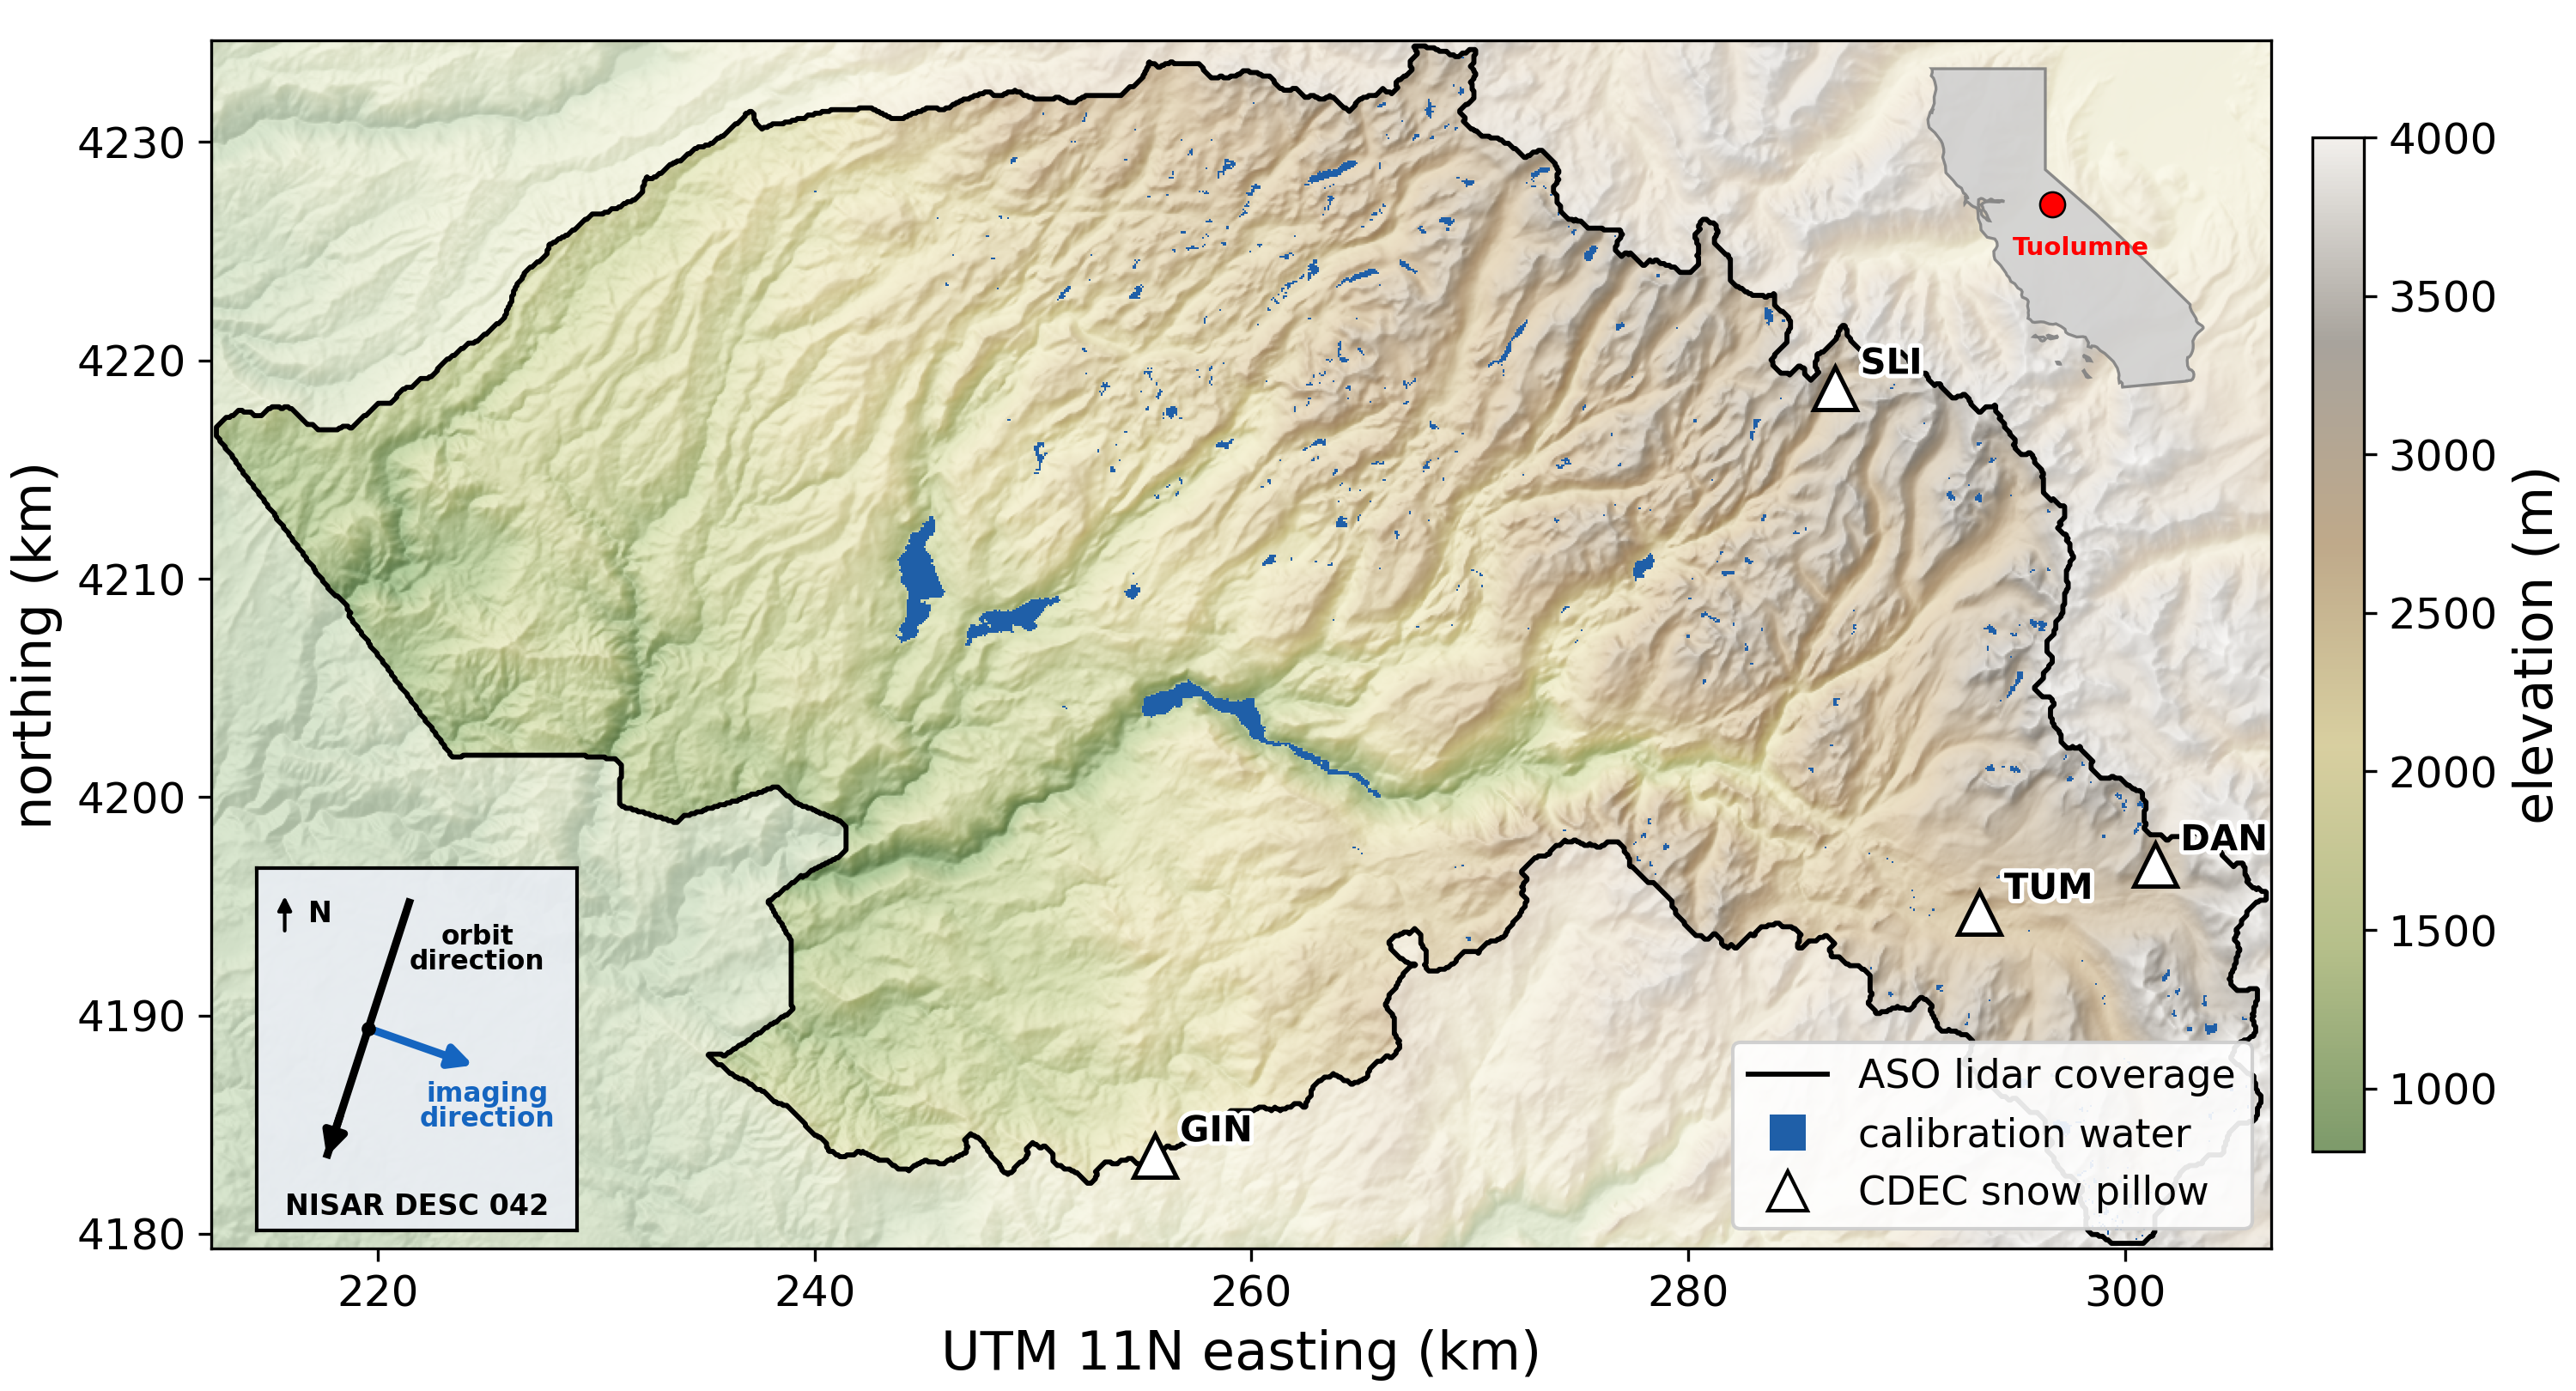
\includegraphics[width=0.5\linewidth]{figures/3_study_area.png}
    \caption{Manuscript's figure 3}
    \label{fig:placeholder_study_area}
\end{figure}

\textit{Discussion: To what extent does the NISAR data being uncalibrated affect this study?}

Very little, because the study uses only the NISAR coherence magnitude and never retrieves phase or SWE from the NISAR products. Since submission, NISAR has released provisional products for both pairs (product version 1.0.11, with RFI mitigation and updated geocoding), and we have redone the NISAR analysis with them. Over the lidar extent the provisional coherence is slightly lower than the beta coherence, by a mean of 0.024 for the December 7--19 pair and 0.009 for the December 19--31 pair, and within each pair the change is the same at the 20 and 80\,m look counts (within 0.001). Recalibrating the effective number of looks over water on the provisional products moves the oversampling factor from 1.29 to 1.32. The corrected $\tilde{\gamma}_{20}-\tilde{\gamma}_{80}$ residual is unchanged for the no-accumulation pair (median $-0.004$) and changes from $+0.031$ to $+0.028$ for the storm pair. The revised manuscript uses the provisional products throughout, and the calibration values, the coherence results, the coherence figure, and Appendix B have been updated (lines 253--258 and 326--327).

\textbf{Technical Corrections}

\textit{Line 32: No comma needed after "acquisitions".}

Removed (line 32).

\textit{Line 36, 45: Consider alternative to having "SWE" as single variable name.}

We considered this but have kept $\Delta$SWE. It is the standard notation in the snow InSAR literature (Guneriussen et al., 2001; Leinss et al., 2015; Oveisgharan et al., 2024). Also, a single-letter symbol would be less immediately clear to the reader. We set it upright, as $\mathrm{SWE}$, so that it reads as one quantity rather than a product of variables.

\textit{Line 125: Specify that 3m and 50m are spatial resolutions, if that is what they are.}

They are. Section 3.2 now says 3\,m and 50\,m spatial resolution where the two products are introduced (line 158).

\end{document}